\documentclass[12pt]{report} % Times New Roman, 12pt
%\usepackage{gscale_thesis_singlespace} % Single spaced thesis
\usepackage{gscale_thesis_doublespace} % Double spaced thesis
\usepackage{fancyheadings} % Header and footer styling
\usepackage{natbib} % Bibliography formatting
\usepackage{setspace} % Allows double spacing but skips headers/footers
\setcounter{tocdepth}{1} % Limits the TOC to chapter and section names

% Additional packages
\usepackage{graphicx} % Allows the inclusion of figures
\usepackage{subcaption} % Allows captions to be added to subfigures
\usepackage[justification=centering]{caption} % Centres caption text
\usepackage{array} % Used for table formatting
\newcolumntype{P}[1]{>{\raggedright\let\newline\\\arraybackslash\hspace{0pt}}m{#1}}
\usepackage{booktabs} % Fancy-style tables
\usepackage{longtable} % Allows for tables that are more than one page long
\usepackage{float} % Better figure placement control
\usepackage{enumerate} % Numbered lists
\usepackage[shortlabels]{enumitem} % For controlling enumerate labels
\usepackage[shortcuts]{extdash} % Allows manual hyphenation of hypenated words
\usepackage{amsmath} % Non-standard math symbols
\usepackage{amsfonts} % Extended fonts for mathematics

\usepackage[hidelinks]{hyperref} % Linking to LaTeX labels and external URLs

\numberwithin{equation}{section} % Numbers equations based on their section

% ********************************
\begin{document}
\title{Your Thesis Title, Which Can Be As Long As You Want On the Title Page}
\halftitle{Short Title} % 60 Characters Max. Including Spaces

\author{Jane Doe}
\shortauthor{J. Doe} % Used for page header

\dept{Department You Belong To}
\field{Your Field} % What field your thesis is in (e.g. Software Engineering)

\prevdegreeone{B.Eng. (Software Engineering \& Game Design),\\ McMaster University, Hamilton, Canada}
\prevdegreetwo{B.Eng.} % Just your degree's field

\submitdate{MONTH YEAR} % Use the month's full spelling e.g. November
\copyrightyear{YYYY} % Year you are submitting this, usually your graduation 
%year

\doctype{Report} % ``Report'' or ``Thesis'' or whatever you need
\degree{Masters of Engineering} % The degree you get when you submit this
\degreeabbrv{M.Eng.}
\principaladviser{Your Supervisor} % Your Supervisor
 % LaTeX variables for preface pages/headers
    
\beforepreface % Half title page, title page, declaration page   
  \prefacesection{Lay Abstract}

A lay abstract of not more 150 words must be included explaining the key goals and contributions of the thesis in lay terms that is accessible to the general public.  % Lay Abstract
  \prefacesection{Abstract}
Drasil is a framework that generates software, including code, documentation, software requirement specification, user manual, and axillary files. Recently, the Drasil team has been interested in expanding its knowledge to solve higher-order ODEs. In this research, for single higher-order linear ODEs, the Drasil framework can solve them without manually extracted information. For higher-order nonlinear ODEs, the Drasil framework can solve them with manually extracted information.

Firstly, we design a flexible and reusable structure to store ODE information based on conventional mathematical knowledge. This makes it possible to reuse ODE information for documentation and for code generation. Secondly, we provide a commonality analysis of four external ODE solver libraries. The analysis includes how they solve the ODE, what algorithms they use, and what options they provide for different types of output. Thirdly, we enable the Drasil Code Generator to solve nonlinear higher-order ODEs with some manually extracted information. We created a new case study, Double Pendulum, that has a system of higher-order ODE. Further, we solve the Double Pendulum example numerically via external libraries. Lastly, for single higher-order ODEs, the Drasil Code Generator can generate code without manually extracted information.

This research accomplishes three main goals. Firstly, we capture the knowledge of linear ODE in a flexible and reusable structure. Secondly, we expand the Drasil capability to solve higher-order ODEs with/without manually written equations. Solving single higher-order linear ODEs does not require manually extracted information. To solve nonlinear ODEs, manually extracting information from the original ODE is still required. The last one is removing the duplicated information caused by the implementation of solving ODEs. % Abstract
  %\thispagestyle{empty}
\null\vfill
\begin{center}
%\textbf{Dedications}
%\linebreak
\textsl{Your Dedication \\ Optional second line}
\end{center}
\vfill
 % Dedication
  todo
 % Acknowledgements
  \referencepages % Table of Contents, List of Figures, List of Tables
  \prefacesection{Notation, Definitions, and Abbreviations}

\section*{Notation}
\begin{description}[font=\rmfamily\bfseries, leftmargin=3.5cm, style=nextline]
	\item[$\mathbb{R}$] any real number in (-$\infty$, $\infty$).
	\item[$\mathbb{R}^n$] a sequence that contains real numbers, n depends on number of inputs values.
	\item[$\mathbb{R}^i$] a finite sequence that contains real numbers, i depends on the start time, end time, and time step.
	\item[$\mathbb{R}^j$] a infinite sequence that contains real numbers, j is a natural number.
	\item[$\mathbb{R} \rightarrow \mathbb{R}^k$] a function takes an independent variable and outputs a sequence of dependent variables.
\end{description}

\section*{Definitions}
\begin{description}[font=\rmfamily\bfseries, leftmargin=5cm, style=nextline]
	\item[Drasil Framework] references the whole \href{https://jacquescarette.github.io/Drasil/}{Drasil Project}.
	\item[Drasil Code Generator] compile captured knowledge to code.
	\item[Drasil Printer] displays captured knowledge in SRS.
\end{description}

\section*{Abbreviations}
\begin{description}[font=\rmfamily\bfseries, leftmargin=3.5cm, style=nextline]
	\item[ACM] Apache Commons Maths
	\item[BDF] Differentiation Formula Method
	\item[BVP] Boundary Value Problem
	\item[DblPendulum] Double pendulum
	\item[GOOL] Generic Object-Oriented Language
	\item[IVP] Initial Value Problem
	\item[NoPCM] Solar water heating system without PCM
	\item[ODE] Ordinary differential equation
	\item[PDController] Proportional derivative controller
	\item[RK] Runge-Kutta
	\item[SCS] Scientific computing software
	\item[SglPendulum] Single Pendulum
	\item[SRS] Software requirements specification
\end{description}
  \academicstatement{academicachievementdeclaration}
\afterpreface
  

  \chapter{Introduction}
\label{chap:introduction}

\begin{writingdirectives}

      \item Move 1: Establishing a research territory by:
      \begin{itemize}

            \item showing research area is important, interesting, and
                  incomplete

            \item reviewing previous research

      \end{itemize}

      \item Move 2: Establishing a niche by noting gaps in previous research.

      \item Move 3: Occupying the niche by:
      \begin{itemize}

            \item outlining purpose

            \item listing research questions

            \item announcing principal findings

            \item stating the value of the previous research

      \end{itemize}

      \item General Structure:
      \begin{itemize}

            \item Introduction:
                  \begin{itemize}

                        \item Jazzy information to get reader hooked

                        \item States purpose of chapter

                        \item Roadmap of what will be discussed in chapter

                  \end{itemize}

            \item Background: context of research problem, sets up the need for
                  research and relevance

            \item PPSQ: should be within first 3 pages of thesis, after intro +
                  background information.

            \item Research design and context: description of where the research
                  takes place (Drasil), introducing methodology briefly

            \item Assumptions, limitations, scope of research, and expected
                  outcomes: what do we need from this work

            \item Overview of chapters

      \end{itemize}

      \item Last Paragraph: summarize key points of chapter, link to next
      chapter

      \item What is the context of this research? What is it about?

      \item What problem does this research tackle?

      \item Why is the research problem important/significant?

      \item What previous research exists?

      \item What is the purpose of this research? What are the goals?

      \item What did the author contribute?
      \wqanswer{\Cref{sec:intro:contributions}}

      \item What does this thesis contain? \wqanswer{\Cref{sec:intro:outline}}

\end{writingdirectives}

\intodo{Add links to where these above writing directives were derived from.}

The usual means of building software involves multiple artifacts (such as
specifications and code) that contain duplicate information that is also
supposed to be linked (\textit{traceability}). Drasil aims to use a generative
approach to de-duplicate this information and make traceability more immediate.

For any ``software'', its artifacts (such as specifications and code) are linked
together by a common thread of knowledge. This knowledge typically ends up used
in the production of the software artifacts, and, often, appears in different
forms and is duplicated, in the produced artifacts. Drasil\cite{Drasil2021} aims
to use a generative approach to de-duplicate this information and make the
\textit{traceability} of knowledge more immediate. Drasil currently studies
generating \ACF{scs} conforming to a \ACF{srs}. This work aims to

As the world increasingly relies on software and non-executable software
artifacts, the software becomes increasingly scrutinized in multiple facets.
Does a piece of software do what I want/need? Is it stable? Is it reliable? What
methods does it use? What do its components mean? Are its outputs accurate and
precise? Is it performant? Is it efficient? Further, to each answer, one might
ask: How do we know? Often, we look to the source code and its development to
justify responses to these questions. Where a requirements specification and a
software design is built, we can spend time investigating that the source code
conforms to the manuals, and that the manuals form satisfactory answers to our
questions. Where a manual is not built, we must spend time studying source code
to respond to these questions, perhaps even comparing them to a control group
program. However, this is terribly arduous process. Realistically, the answers
to these questions should have been already well-understood before the final
software product was formed, even if the answer was to ignore the question until
later. Drasil \cite{Drasil2021} looks to form answers to these same questions
through \textit{definition}. Using generative techniques, Drasil builds software
that conforms to specifications by having all relevant information of the
specifications and how they translate into some software artifacts
well-understood to Drasil. This thesis aims to explore these ideas through
exploring capturing mathematical knowledge in Drasil.

\section{Problem Statement}
\label{sec:intro:problemStatement}

Drasil has de-duplicated knowledge across \acs{scs} artifacts relevant to
specifications and code. Through codifying knowledge and collecting a coherent
set of information in a knowledge database, we are able to generate a wide
variety of software artifacts (e.g., \acs{oo} programs [Java, C$++$, Python,
            Swift, and C\#] with guided usage via Makefiles, and requirements specifications
      [HTML and TeX]). This codified knowledge was de-duplicated from an originating
set of artifacts via bottom-up gathering, however, we should be able to use the
same knowledge to generate more artifacts in different languages, flavours, and
with more options. However, each desired artifact language has its own way of
encoding information (such as mathematical expressions). This leaves us needing
to teach Drasil more about the targeted languages (and, at times, about the
existing codified knowledge) in order to reliably generate usable artifacts.
Mathematical expression and theory encoding becomes a key point of interest for
us because they are used in across the board (e.g., derivations, code,
constraints, definitions, etc.). Drasil relies on a single universal untyped
mathematical language to describe general mathematical knowledge (theories).
Unfortunately, this results in unreliable and brittle conversions of
mathematical knowledge into other forms because, we, lack information about
their structure (leading to inflexible conversions to other forms), don't
statically know when expressions are admissible in different contexts (e.g., in
code generation, derivations, etc.), and we don't know when are well-formed
(well-typed). As more theories are codified and typed, Drasils knowledge
database faces difficulties in scaling since it relies on a single unique map
for each type of knowledge, resulting in an ever-growing list of maps and a
tediously precise means of knowledge collection and reference.

\section{Research Questions}

\begin{enumerate}

      \item[\namedlabel{rq:one}{RQ1}] Drasil has a language of simple
            mathematical expressions that are used in multiple contexts. But not
            all expressions are valid in all contexts. How do we fix that?

      \item[\namedlabel{rq:two}{RQ2}] Drasil's current encoding of "theories"
            are essentially black boxes. We would like to be able to use some
            structural information present in the short list of the ``kinds'' of
            theories that show up in scientific computing. How do we codify
            that?

      \item[\namedlabel{rq:three}{RQ3}] How can we ensure that our language(s)
            of simple mathematical expressions admits only valid expressions?

      \item[\namedlabel{rq:four}{RQ4}] Our current ``typed'' approach to
            collecting different kinds of data is hard to extend. How can we
            make it easier to extend?

\end{enumerate}

\section{Contributions of the Author}
\label{sec:intro:contributions}

\intodo{\ref{rq:four} Link each sentence in the contributions section to the
      rqs.}

Dr. Jacques Carette built a prototype solution\todo{Cite appendix entry of
      code?. How should I cite what Dr. Carette had already written?} for the
issue of transcribed theories in Drasil not exposing enough information
for reliable code generation (as discussed in \Cref{chap:modelkinds}).
Relying on Dr. Jacques Carettes prototype, A current implementation and
other re-designs in the works have been developed by the author of this
work. Both issues discussed in \Cref{chap:modelkinds} and
\Cref{chap:typedExpr} were discussed before the author had joined the
Drasil research group. Drasil, and the expression language in particular,
had been constructed before this work.

\section{Thesis Outline}
\label{sec:intro:outline}

In \Cref{chap:ideology}, we discuss the focal ideology underpinning this work
and Drasil. \Cref{chap:drasil} describes Drasil, the host project carrying the
fruits of this work. \Cref{chap:modelkinds} discusses how theories are encoded
in Drasil, the issues associated with using a single universal mathematical
language to describe theories, and how we can resolve these problems.
\Cref{chap:typedExpr} describes residual issues associated with validating and
transcribing mathematical expressions. \Cref{chap:storingChunks} continues to
discuss the ways in which general knowledge and theories are encoded in Drasil,
and methods for altering their encoding, leading into \cref{chap:futureWork},
where we discuss future work.

\chapter[Ideology]{Ideology\footnotemark}
\footnotetext{Or, at least, my understanding of a software development ideology
    I believe to be relevant to this work.}
\label{chap:ideology}

``Generation'' is at the heart of this work. However, unlike GitHub and OpenAI's
Copilot \cite{Copilot}, we don't delve into artificial intelligence. Copilot
uses AI to autocomplete code using smaller snippets and comments, while we focus
on capturing the meaning of specific subsets of language to generate software
artifacts through description of their requirements. In other words, we focus on
encoding the important bits of information that we use to discuss requirements
of software and how they relate to the software artifacts we would normally
manually write. Succinctly, we focus on capturing knowledge through codifying
well-understood fragments with \acsp{dsl}, which we use to improve
\textit{reusability} and \textit{maintainability} of software by improving
knowledge sharing and usability, and creating a more \textit{harmonious
relationship} between our \textit{knowledge} and \textit{software artifacts}.

\section{On Developing Software}
\label{chap:ideology:sec:on_developing_software}

As software developers, we encode ``stories'' through software. As an example,
programs made to process \acs{csv} files tell a story of how data can be
entered, adjusted, and output. Compilers tell a story of how human-readable
programs can translate to various assembly languages. In these stories, we
commonly use similar terminology and ideas. Thankfully, we avoid writing ``a lot
of the same code'' by abstracting over variables and sharing reusable code
through libraries. With libraries, we're able to share our knowledge with our
future selves and others alike. Once we've reasonably stabilized our libraries,
it becomes a large gain in the reusability of our efforts \textemdash we don't
need to worry about making the same bugs twice! However, a few issues arise: the
code might become out-of-date (or out-of-sync), others might not understand what
we wrote (and, thus, not trust/use it), or, we might need to use the same
conceptual ideas but in a different programming language. If our understanding
of key ideas changes, we might need to perform large, manual, refactoring of our
code, and then update our documentation too. While we might write ``idiomatic''
code, reverse engineering code is tedious, and even then, we can only analyze
the code we \textit{see}, and not what knowledge it took to write that code.
Finally, we might be able to write a \ACF{ffi}, but they're often brittle and
demanding of our time, due to initial and repeated complex analysis for each
library update. We might even be forced to use particular programming languages.

Often, we look to using mature libraries and frameworks to underpin our
projects, but usually without a guarantee that how we use and connect libraries
is ``safe.'' For example, the sinking of the Vasa ship \cite{wiki:Vasa_ship} was
partially caused by different teams working together but using different
``feet'' units (the Swedish foot is 12'' while the Amsterdam foot is 11'')
resulting in unbalanced weight distribution, contributing to its demise.
Similarly, when the Mars Climate Orbiter travelled to Mars, it met an early
demise due to a navigation issue \cite{Siddiqi2018}. Lockheed Martin built the
orbiter ground controller software, but it didn't conform to \acsp{nasa}
\ACF{sis}. The commands sent from Earth used English units (specifically,
pound-seconds) while the orbiter assumed that it would receive commands using
the metric system (Newton-seconds). As such, the orbiter missed its intended
target orbit altitude, falling into the Martian atmosphere, and ultimately
disintegrating due to atmospheric stress.

Experts had an in-depth understanding of the ``story'' of each project, with
sound rationale for how things worked and should have worked, and yet, both
ended in misfortune. Of course, most software is not critical, and issues in
most software will not result in an orbiter disintegrating in Martian atmosphere
or a ship sinking, but, there is something that we can learn:
\textit{communication} and \textit{synchronization} of development efforts is
vital for building reliable solutions.

While we, as developers don't often build and connect physical things, we do
connect pieces of code\footnote{Though robotics is a field too.}, but
misunderstandings of tacit project knowledge occur too. Thus, we believe we need
to revisit our original sensation when we recognized code duplication and
decided to make reusable components.

The reason is obvious\footnote{Ignoring the more obvious reasons, such as
copy-pasting code, or mere awareness of textual similarities.}! We felt this
sensation because we already had a mental model that connected some key concepts
to some code we wrote, so we decided to make reusable views (code) of our
knowledge. However, the code is only a shallow view of our knowledge, containing
very little discussion of the conceptual underpinnings and the role they play in
the greater ``story.'' Shallow views of implicit, unwritten knowledge,
unfortunately, does not come with guarantee of harmony with the way it's used.

\section{Dreams of Generation}
\label{chap:ideology:sec:thoughts_of_generation}

Unlike the Vasa, for stories where the desired end-product somehow involves
software, we can remedy the communication issue partially by unifying it under
one cohesive story. \Acfp{srs} play a large role in unifying communication of
software needs. However, the communication and maintained synchronization of the
software requirements into the final software product is still brittle (as
evidenced by the Mars orbiter), as it remains heavily reliant on manual labour
to translate it into software artifacts. In other words, the translation from
our knowledge (the important part) is laborious and prone to error, and, hence,
not simple enough. So, now we wonder: how can we simplify the process?

Our end-goal should be ``assembly-line'' style engineering of the software
\cite{well-understood}, free of logical issues. To attain this, we need to have
clear criteria for what it means for our software artifacts to be free of
logical issues. However, to do this, we need to discuss relevant models. For
example, if we're interested in the accuracy of a bank accounts cached balance,
we discuss \textit{the user}, the relevant \textit{transactions}, and then a
\textit{validation algorithm}. Realizing this example in code might have us
retrieve a user's bank transactions, calculate the expected balance, and compare
it with a cached balance. The code only contains one dimension of this
discussion: the actions, it has no understanding of the substance, nor how it
can be similarly used in other scenarios. To audit the code, we analyze the code
ourselves, potentially with extra testing tools to make things quicker, but, in
general, it relies on us and our understanding. To remedy this, we look to
describing software as we've done here: as a ``view'' of some story or
discussion. In other words, we want to build software artifacts through
description as opposed to manual conversion of description to artifact.

\subsection{The Goal}
\label{chap:ideology:sec:thoughts_of_generation:subsec:the_goal}

If we think of a Java compiler as a sort of \textit{generator} of \acs{jvm}
bytecode, we can think of the Java programs as the instructions and inputs to
the generator. We rarely look at the actual bytecode ourselves, but we do have
confidence in knowing what it will do when executed. Now, we look to go one
``level'' up. In other words, we look to inputting our understanding of
particular applications through another generator (an abstraction level up) to
somehow obtain code for it.

Especially in the cases where everything is ``well-understood''
\cite{well-understood}\footnote{Irrelevant of rarity!}, we want to focus on
communicating problems and how solutions solve them so that we can
\textit{generate} usable solutions (a software artifact), and keep them
up-to-date through re-generation.

\subsection{Reconciliation}
\label{chap:ideology:sec:thoughts_of_generation:subsec:reconciliation}

By focusing on capturing well-understood \cite{well-understood} knowledge, we
can use (and re-use) knowledge across specialized generators to generate
software for specific kinds of problems. For example, statisticians frequently
use and discuss various kinds of distributions, such as ``Poisson,''
``Uniform,'' and ``Normal,'' and, when they do, they're typically familiar with
their parameters, expectations functions, and how to use them to estimate
likelihoods. Hence, by focusing on using \textit{\acsp{dsl}}, we can build
specialized interpreters for them. Furthermore, by connecting them in precise
manners (with similar precise languages), we can form large meaningful
\textit{networks of domains} \cite{Czarnecki2005} that form our well-understood
problem spaces. For well-understood problem spaces, we can compose a series of
domain-specific interpreters. With enough effort, we could take a whole
``problem description'' that draws in multiple fields, and generate software
that somehow ``solves'' it.

By switching our focus of manual software development to manual problem
description and relationships to ``solutions,'' we shift where we can make bugs,
and how they propagate. Namely, logical bugs will occur more than once so as
long as the same knowledge pulled from is drawn more than once. Thus, each
logical bug should be more visible and easier to spot. Additionally, the
generated software becomes directly \textit{traceable} to its logical
foundations. Hopefully, with adequate dissection of related concepts, bugs
should also be less intricate. Furthermore, generated artifacts are simpler to
\textit{maintain} (i.e., kept in synchronization) with its related
knowledge-base and story by \textit{regenerating} it. Finally, as opposed to
sharing \textit{code}, in this paradigm, we \textit{communicate knowledge},
achieving language-agnostic reusability, focusing on sharing meanings and
families of problems rather than solutions. Thus, by focusing on generating from
meaningful descriptions, we obtain \textit{knowledge reusability} (as opposed to
\textit{code} reusability), and increased software \textit{maintainability},
\textit{reliability}, and \textit{traceability}. Of course, ``generating
everything'' appears grandiose, and, perhaps, reductive or ignorant of many
difficulties in software development. Thus, we must discuss
feasibility\footnote{You may skip the remainder of this chapter if you so wish,
it is not strictly required to understand the rest of my work, but it doesn't
hurt.}.

\subsection{Feasibility}
\label{chap:ideology:sec:thoughts_of_generation:subsec:feasibility}

For us to discuss feasibility of this idealized development paradigm, we must
discuss the \textit{depth} and \textit{breadth} of knowledge we need to make
this feasible\footnote{Note that ``knowledge'' is captured through codifying
\acsp{dsl}.}. Depth of knowledge refers to the vertical knowledge understood
about a specific fragment of knowledge, and its preciseness. For example, we may
have a low-depth of knowledge and claim that English sentences are a sequence of
characters. Alternatively, we might have a slightly ``deeper''
depth/understanding  of sentences by describing them as a language that follows
a specific syntax rule set and using a specific set of words. Breadth of
knowledge is the horizontal domain of knowledge, it is the various kinds of
knowledge we have in a wide variety of subjects and domains.

\subsubsection{Bottom: The Lowest Depth \& Narrowest Breadth}
\label{chap:ideology:sec:thoughts_of_generation:subsec:feasibility:subsubsec:bottom}

In some sense, at the lowest depth and narrowest breadth of knowledge capture,
we aren't really capturing any meaning. Rather, we are programming our software
artifacts directly. Hence, this area is already very feasible, as evidenced by
the usefulness of software today and the way it was made.

\subsubsection{Shallow Waters: Low Depth \& Narrow Breadth}
\label{chap:ideology:sec:thoughts_of_generation:subsec:feasibility:subsubsec:low}

At a shallow depth and relatively narrow breadth of knowledge capture, this
paradigm is very practical, and already heavily used. Widely used \ACFP{cms},
such as WordPress \cite{WordPress} and Drupal \cite{Drupal}, and web frameworks,
such as Django \cite{Django} and Laravel \cite{Laravel}, are arguably also
following similar ideals as this ideology. Notably, they \textit{deeply embed}
\cite{Carette2009} knowledge in their frameworks and libraries using their host
programming languages basic features. They all typically provide a basic
understanding of ``user's'' of a hosted website, facilities to write \acs{html}
content in one way or another (e.g., \acs{wysiwyg} editors, templates, and
plugins). While some might be, these listed above are not specific to one
specific use-case. They're versatile products, usable for a wide variety of
use-cases because they ship with low but sufficient depth of
knowledge\footnote{They might call it ``features.''} such that you can use them
for a wide variety of different applications (e.g., blogging, ticketing,
booking, accounting, etc.). Out of the box, these web technologies listed come
with simple, common, functionality (features) and powerful extensibility through
either plugins or through software extension and usage. With the basic tooling
provided, users are able to rapidly deploy websites with content. Through
extending the website's knowledge-base (e.g., plugins or software extension),
they are able to obtain a wider breadth and deeper depth to the knowledge
contained within them. Through this, end-users may encode increasingly complex
and different kinds of data into the systems to ultimately obtain increasingly
specialized websites, such as technical blogs, eCommerce websites, online
accounting software, online discussion forums, and more.

The mechanized generation-related components of the ideology is also fairly
shallow in this area, but, still, highly feasible. In some sense, almost any
individual instance of ``generation'' is an area of low depth and breadth as
well.

\subsubsection{Specialization: Deep Depth \& Narrow Breadth}
\label{chap:ideology:sec:thoughts_of_generation:subsec:feasibility:subsubsec:specialization}

We might think of software that captures deep knowledge about a specific topic
as \textit{specialized tools}. Tailored to specific needs, they come with extra
features for highly specific, potentially niche, categories of
problems\footnote{Think of this category as sharp tools, such as kitchen knives.
We can generally get away with using basic kitchen knives, but specialty knives
help us out for particular use-cases, such as serrated knives or filleting
knives.}. These already exist, and are, similar to the ``Bottom,'' highly
practical. For example, \ACFP{aml} (such as HashedExpression
\cite{HashedExpression}) allow you to describe complex mathematical algorithms
and generate optimized software tools for solving them. Another example is
parser generators (such as Happy \cite{Happy}). They capture complex information
about grammars and allow users to generate specialized parsers for them. When
needed, specialty tools provide greater functionality than general-purpose
programming languages for solving specific problems.

\subsubsection{A Wide But Shallow Reaching Net: Low Depth \& Wide Breadth}
\label{chap:ideology:sec:thoughts_of_generation:subsec:feasibility:subsubsec:modelling}

Orthogonal to the ``specialized tools,'' a capture of low depth and wide breadth
of knowledge is seemingly a jack of all trades, master of none. For example,
most modern programming languages come with a standard library that provide many
off-the-shelf solutions to well-understood problems, but sticking to very common
generic problems. Most users typically pull in a library that provides extra
specialization for certain problems because the standard library didn't go deep
enough for their needs. Similar to the categories before, these are widely used
and similarly practical.

\subsubsection{Utopia: Deep Depth \& Wide Breadth}
\label{chap:ideology:sec:thoughts_of_generation:subsec:feasibility:subsubsec:utopia}

Finally, we've reached the category of ``deep depth and wide breadth'' of
knowledge capture. Here, we capture the meanings of key ideas and concepts we
need to build software, making as many conscious decisions explicit and visible
as possible. Imagine using the specialized tools to develop every aspect of some
software artifact, but for every facet of the artifact, from start to finish.
This is an idealized method of developing software, where knowledge is strongly
reusable and composable. Of course, this relies on heavy research on tooling. As
long as developers have infinite patience and can invest infinite time into
transcribing and researching to fill in gaps, anything is possible, and this
ideology is very practical! Unfortunately, that situation is not quite
realistic. As such, we should restrict our scope of captured knowledge to
``well-understood'' domains \cite{well-understood}. For areas of
``well-understood'' knowledge, this should be more feasible, merely because the
discussion of key ideas is already coherent and sufficiently codified.

Here, you might use a series of \acsp{dsl} to create a coherent discussion (a
``story''). With it, you would have specialized interpreters built, which
process it, and draw out meaningful byproducts you're interested in (such as
usable software). This story can be relatively far removed from produced
artifacts generating (containing potentially little to no discussion of the
desired artifacts at all), or a precise description (where you might be manually
writing out the final artifacts yourself). Through creating a story as a
composition of many other smaller fragments of knowledge and stories, and
defining interpreters as compositions of other, smaller, interpreters, this is
feasible. Hopefully, with enough effort, this should alleviate considerable
stress associated with manual software development, by moving the focus to the
important bits: the story the artifacts tell. The ``quality'' of the generated
artifacts become a traceable reflection of the ``quality'' (depth and breadth)
of the captured knowledge.

\section{A Prospective Workflow}
\label{chap:ideology:sec:a_prospective_workflow}

In theory, all ``development'' should occur in a \ACF{kms}, where knowledge and
transformations between fragments of knowledge are transcribed. ``Users'' would
use a system of pre-filled knowledge to piece together a template story that
fits their narrative, or they would adapt an existing one to fit theirs.

Ideally, the workflow associated with building some product artifact will have
each knowledge/product owner (e.g., actual property ``\textit{owner}'',
developers, managers, designers, etc.) work on strictly the components that are
related to them, and nothing else. At the ``bottom'', the final end-user is
tasked merely with providing feedback that can improve the quality of the
artifact(s). They are the ones that have an issue that can be resolved with some
sort of software artifact. At the ``top,'' product owners designate a basic set
of requirements of the artifacts using a coherent \textit{formal description}.
Product designers/orchestrators will take the requirements and convert them into
a coherent \textit{story} for how the requirements may be translated into a
final product. The story builds on well-understood knowledge of various domains
encoded by domain experts. The product designer is tasked primarily with
translation, while the domain developers and product owners are tasked with
encoding knowledge and instances of knowledge, respectively.

Through product owners describing their requirements coherently (e.g., via some
formal language), completely non-technical product owners may, and will, still
be key figures in the production of the product.

As the stress load/burden becomes shared under this paradigm, the sum of the
parts should be less than the whole. In other words, the cumulative stress of
associated with creating the whole is greater than the approximate sum of each
individual's stress associated with focusing on their respective domain.

Following this ideology, there will be at least 3 key roles associated with
developing artifacts: the \textbf{knowledge encoder}, the \textbf{knowledge
user}, and the \textbf{end-user} of the produced software artifact.

\subsection{Knowledge Encoder (Domain Expert)}
\label{chap:ideology:sec:a_prospective_workflow:subsec:knowledge_encoder}

The knowledge encoder should be a master of a particular domain. They are
expected to encode the knowledge discussed in their respective domain in such a
way that is accessible to those without knowledge of their domain. Additionally,
they should encode information about the ways in which the knowledge can be
transformed into other forms of knowledge (including that which is
interdisciplinary). The knowledge they would be encoding should be as well-known
and globally standardized as possible. As discussed in
\Cref{chap:ideology:sec:thoughts_of_generation:subsec:reconciliation}, it is
likely that the knowledge encoder will focus on writing a series of highly
specific \acsp{dsl}, where the languages may be restricted to as specific as one
term or a handful.

As a domain expert transcribing knowledge encodings of some well-understood
domain, one will largely be discussing the ways in which pieces of knowledge are
\textit{constructed} and \textit{relate to each other}. For the abstract
knowledge encodings to be \textit{usable} in some way, it is vital to have
``names'' (\textit{types}) for the knowledge encodings. In working to capture
the working knowledge of a domain, it's of utmost importance to ensure that all
``instances'' of your ``names'' (types) are \textit{always} usable in some
meaningful way and that the knowledge is exposed in a usable way (e.g.,
sufficiently through some sort of \acs{api}). In other words, all knowledge
encodings should create a stringent, explicit set of rules for which all
``instances'' should conform to, and, arguably, also creates a justification for
the need to create that particular knowledge/data type. As such, optimally, a
domain expert would write their knowledge encodings and renderers in a general
purpose programming language with a sound type system (e.g., Haskell
\cite{Haskell2010}, Agda \cite{Norell2007}, etc.) \textemdash{} preferring ones
with a type system based on formal type theories for their feature richness.

\subsection{Knowledge / Domain User \& Orchestrator}
\label{chap:ideology:sec:a_prospective_workflow:subsec:knowledge_orchestrator}

The knowledge user/orchestrator is tasked with connecting the work of the domain
experts into ``plug-n-play'' stories (arguably, compilers for the end-users to
use). They should also have a working understanding of what the end-user needs,
and how the needs relate to domains of knowledge. As such, they should be able
to encode and reduce friction between knowledge encoded by domain experts and
the goals of product owners.

\subsection{End-user}
\label{chap:ideology:sec:a_prospective_workflow:subsec:end_user}

The final end-user should find the most delight from this ideology. They are the
actual users of the software artifacts, perhaps tweaking the final build of the
software artifacts to be accustomed to their workflow. If the tasks assigned to
the knowledge encoders and the knowledge users are performed correctly, then the
end-user should have strong confidence in the artifacts as they were built with
strict adherence to the knowledge captured at \textit{every step of the way}. As
such, one should confidently expect the final software artifacts to be
completely devoid of unexpected things (including errors, unconformities to
specifications, etc.).

Any of the three (3) user types may use the ``plug-n-play'' stories to describe
problems and generate solutions based on them.

\section{Drasil}
\label{chap:ideology:sec:drasil}

To my understanding, Drasil \cite{Drasil2021} explores this ideology, focusing
on generating scientific software from user-described scientific problems using
Drasil-understood terminology (i.e., ones that a scientific domain expert
previously encoded).

\chapter{Drasil}
\label{chap:drasil}

\begin{writingdirectives}

      \item What is Drasil?
      \begin{enumerate}
            \item What does it do?
            \item Where can we find information about it?
            \item What are its successes?
      \end{enumerate}

      \item How does Drasil work?
      \begin{enumerate}
            \item SRS? Generation?
            \item Specifically, what are its current problems?
      \end{enumerate}

\end{writingdirectives}

\drasilLogoImg{}

\section{What is it? What can it do?}
\label{chap:drasil:sec:what-is-it-what-can-it-do}

Principally investigated by \porthref{Dr. Jacques
      Carette}{https://www.cas.mcmaster.ca/~carette/} and \porthref{Dr. Spencer
      Smith}{https://www.cas.mcmaster.ca/~smiths/},
\porthref{Drasil}{https://jacquescarette.github.io/Drasil/} is a software suite
for generating software for well-understood problems through a knowledge-first
approach \cite{Drasil2021}. Drasil captures the background knowledge involved
with software development to make it \textit{reusable}, improve
\textit{maintainability} of software, and strengthen \textit{traceability}
between desired ``software artifacts''\footnote{``Software artifacts'' being any
      file with a well-defined structure, such as plaintext files, Python code,
      \LaTeX{} code, \acs{html}, or \acs{json}.} and the background knowledge
\cite{SzymczakEtAl2016}. Currently, Drasil focuses on generating software
artifacts for \ACF{scs}, where it has been shown to improve software qualities,
such as \textit{verifiability}, \textit{reliability}, and \textit{usability}
\cite{Smith2018}.

\roughNetworkOfDomains{}

Drasils knowledge-capture approach to software development allows users to
remove themselves from the discussion of ``code'' and focus on the important
bits: the problem the code solves and how ``code'' ultimately relates to
it\footnote{Drasil allows users to ``keep at a safe distance'' from software,
      but only so far as Drasil has encoded the terminology the users rely on for
      conveying their problem to Drasil.}. Drasil relies on a \textit{network of
      domains} \cite{Czarnecki2005} to capture the knowledge required to generate
artifacts for a series of case studies (\refCaseStudiesTable{}) that Drasil
builds and uses to navigate development. Roughly, the network is as per
\refRoughNetworkOfDomains{}, where nodes are the major categories of
domains\footnote{In other words, each node contains its own subdomain as well}
and arrows are mappings between them. The case studies use structured \ACF{srs}
\cite{SmithAndLai2005} abstraction to describe scientific problems and the
background knowledge necessary for developers to manually build software.
Through sufficient capture of the background scientific knowledge\footnote{Such
      as the key theories, input and output variables, and assumptions.}, Drasil
generates software artifacts that solve the precise problem descriptions
(\refCaseStudiesCodeTable{}). One notable success of the knowledge capture is
the reusability of it to regenerate artifacts in different, but similarly
applicable, languages. For example, the \acs{glassbr} case study had
\porthref{software
      artifacts}{https://github.com/smiths/caseStudies/tree/master/CaseStudies/glass}
manually built. Once the knowledge was codified in Drasil, the same knowledge
allows re-creation in \porthref{other
      languages}{https://github.com/JacquesCarette/Drasil/tree/master/code/stable/glassbr}.

\caseStudiesTable{}

Drasil is able to generate a host of \ACF{oo} programming language source codes
through compiling to \ACF{gool} \cite{MacLachlan2020}, which compiles to several
\acs{oo} languages (such as Java, Python, C/C$++$, C\#, and Swift\footnote{Note
      that Swift was not discussed in \cite{MacLachlan2020}, but the renderer was
      built by Brooks as well.}). Drasil also contains renderers for printing
\acs{html} files, Makefiles, basic Markdown (enough for ``READMEs''), GraphViz
DOT \cite{Gansner1993} diagrams, and plaintext, \LaTeX{} documents. \acs{srs}
abstractions are renderable in either \LaTeX{} or \acs{html}.

\section{How does it work? How is it used?}
\label{chap:drasil:sec:how-does-it-work-how-is-it-used}

As mentioned in \Cref{chap:drasil:sec:what-is-it-what-can-it-do}, Drasil relies
on building a tree of knowledge that contains sufficient information such that
software artifacts can be ``grown'' from them. The individual pieces of
knowledge are known as \textit{chunks} and are encoded as either \ACFP{adt} or
\ACFP{gadt}. Drasil, and all knowledge captured in Drasil, is deeply embedded in
Haskell \cite{Haskell2010} \porthref{source
      code}{https://github.com/JacquesCarette/Drasil/}\footnote{The source code
      compiles against \acs{ghc} 8.8.4 \cite{GHC884} and uses \acs{ghc} language
      extensions.}. Each chunk has a \textit{type} which defines its structural
information. Chunks contain information encoded with various \ACFP{dsl}. The
network of domains (roughly, \refRoughNetworkOfDomains{}) is made up of a series
of chunks connecting and discussing one another, similar to how we might discuss
abstract concepts.

The ``coherent \acs{srs} abstraction'' of \refRoughNetworkOfDomains{} is
modelled after the \textit{Smith et al.} formal \acs{srs} template
\cite{SmithAndLai2005}, while the ``scientific knowledge'' higher up is a set of
interconnected chunks (and, hence, \acsp{dsl}). The ``scientific knowledge''
chunks are used to fill in the ``gaps'' of the \acs{srs} template. For example,
if we wanted to encode a variable, \(\hat{q}_{\text{tol}}\), representing a real
number, ``Tolerable load,'' we might write it as
\refOriginalQuantityDictExampleHaskell{}, where it is of type \QuantityDict{}
(\refOriginalQuantityDictHaskell{}), the type of variable encodings.

\originalQuantityDictExampleHaskell{}

\originalQuantityDictHaskell{}

Notably, in \refOriginalQuantityDictExampleHaskell{}, the symbol,
\(\hat{q}_{\text{tol}}\), is built using a \Symbol{} \acs{dsl}. The capture of
domain-specific knowledge is what sets \acsp{dsl} apart from general-purpose
programming languages. Domain-specific abstractions create opportunities for
domain-specific \textit{interpretation and transformation} (e.g., optimization,
analysis, error checking, tool support, etc.) \cite{Czarnecki2005}. For example,
with the symbol for ``tolerable load,'' we have information about the structure
of the symbol itself: that ``q'' has a ``hat'' and a subscript ``tol.'' From
this, we can output the same information in alternative flavours if we desired,
such as plain text, or with Java-compatible naming convention (e.g.,
``qHatTol'').

Drasils \acs{srs} template contains more ``holes''\footnote{Or ``blanks'' if you
      think of the template as a ``fill-in-the-blanks'' puzzle.} for other
information necessary to creating a whole ``story'' about how
\textit{output variables} can be calculated according to a set of
\textit{input variables} and algorithm derived through a series of
\textit{theories}. With sufficient knowledge \textit{depth}\footnote{Note
      that the \acs{srs} template provides the \textit{breadth} needed by
      design!} for each relevant fragment, Drasil is able to automatically
``check'' it for consistency and coherence, and generate representational
code\footnote{``Representational code'' meaning software that solves the
      problem the related \acs{srs} abstraction describes, using the algorithm
      outlined.}.

Unfortunately, not all of Drasils case studies are capable of generating
representational code (\refCaseStudiesCodeTable{}). Some case studies
(\acs{gamephysics}, \acs{hghc}, and \acs{ssp}) are still actively being
developed, but are left incomplete at the time of writing. \acs{nopcm} is usable
in all languages supported by \acs{gool} except for Swift due to the lack of a
Drasil-supported \acs{ode} solving library for the Swift \acs{gool} renderer.
\acs{pdcontroller} was built \cite{DrasilPR2289Naveen} outside  the normal means
of Drasils case studies development. Code generation for \acs{pdcontroller} is
not impossible, it just requires more investigation by a domain expert for the
needs of the case study. However, both the issues related to \acs{nopcm} and
\acs{pdcontroller} are outside the scope of this work. In this work, we will
focus on a critical common denominator between all examples: capturing
mathematical knowledge for reliable \acs{srs} artifact generation. In
particular, we will focus on 2 primary aspects of mathematical knowledge: the
\textit{theories} and the \textit{expressions}.

\caseStudiesCodeTable{}

% ModelKinds -- Theory types / discrimination -- ``Expressions in context''

In working to understand some phenomenon, we often look to the boundaries of our
understandings of the phenomenon — the open-ended questions and gaps in our
knowledge. In any domain of knowledge (such as mathematics, philosophy, physics,
chemistry, biology, computer science, or any other studied subject), we often
think about various phenomenon in logical terms of theories and axioms, where
the theories and axioms are written using a global logical language with precise
meanings\todo{I almost make it sound like we're not using English/Any other
	language to communicate ideas, I should clarify this.}. The language is
typically tailored to the field of knowledge. As this work pertains to Drasil,
one language of interest to this research is that of the mathematical language.
A mathematical language is heavily used in science, conveying important
theories, axioms, corollaries, amongst other things. As mathematicians
transferring knowledge to one another, we often use a written form of knowledge,
though unlikely, potentially, with a precise structure to our transcription of
the knowledge, but still, the structure is textual. We might break up the
transcription of the knowledge into sections. The sections of a theory may have
a name, a natural language description, a derivation, some information regarding
its origin (e.g., a reference), and a formalization of the theories important
information in a precise language. Of course, for a mathematical theory, a
mathematical language would be used. Describing a programming language artifact,
we might prefer to call our theories by a series of other names (e.g.,
functions/methods, constants, modules, packages, libraries, \acsp{api},
\acsp{ast}.

In Drasil, both of these languages are of great importance. The mathematical
field of knowledge is directly used in at least two domains currently captured:
the scientific theories, and \acs{gool} \cite{Carette2019}. Meanwhile, the
programming language theory (artifacts) is only directly used in \acs{gool}, and
its various renderers. The SmithEtAl \acs{srs} \cite{SmithAndLai2005} template
generator uses knowledge transcribed as scientific requirements to automatically
generate a series of representational software programs. Thankfully, Smith and
Lai \cite{SmithAndLai2005} break down theories relevant to \acs{scs} into at
least four (4) kinds for their \acs{srs} template:

\todo{Define the 4 kinds of models here.}
\begin{enumerate}

	\item \textbf{Theory Models}:

	\item \textbf{General Definitions}:

	\item \textbf{Instance Models}:

	\item \textbf{Data Definitions}:

\end{enumerate}

\intodo{Example of a theory/instance model here.}

\intodo{Insider knowledge: the theories are actively being re-thought.}

Since the SmithEtAl generator focuses itself on knowledge captured in the form
of the \acs{srs} template, Drasil requires a comprehensive understanding of both
fields in order to generate representational software for the \acs{srs}. The
focus of the scientific requirements documents are to transcribe the relevant
knowledge of a \acs{scs} system as developed by a domain/scientific expert. For
example, \todo{SRS document example} is used to fully explain \todo{something}
such that a software developer can construct a program based on it. Of course,
if the \acs{srs} document is to be truly sufficient for a software developer to
unambiguously create a representational software artifact, then the software
developer (who potentially knows nothing about the domain discussed in the
\acs{srs} document) will need to be able to credibly transcribe everything into
their program, matching the requirements as set by the \acs{srs} document.
Drasil is an apparatus for testing our understanding of these scenarios, rather
than having a read-only ``view'' of the scientists/domain experts knowledge
available to the software developer, the knowledge itself is available, in its
most raw encoded form.

Drasil relies on searching for a calculation path that relates the inputs and
outputs designated in an \acs{srs} document. The relations are based on the
grounded theories (\textit{Instance Models}) designated in the \acs{srs}. The
relations themselves are currently required to be of the form \(x = f(a, b, c,
\ldots{})\), with some exceptions made for \acsp{ode}. \acsp{ode} are being
actively developed to remove the manually written exceptions made for them
(outside the scope of this work).

Instance Models, General Definitions, and Data Definitions each rely on a
\textit{Relation Concept} (\RelationConcept{}): a notable and named mathematical
relation with a description and abbreviated name. A \RelationConcept{} is
modelled as a \Relation{} coupled with a \ConceptChunk{} (\todo{Add ConceptChunk
	original definition to thesis appendix.}, a named \textit{thing} with a name,
abbreviation, and natural language description):

\originalRelationConcept{}

The \Relation{}s \todo{add a reference to an appendix entry for the ``type
	Relation = Expr'' definition} in the \RelationConcept{} are, fundamentally,
just an instance of a universal mathematical language which conveys their
information, but given a type synonym to indicate that the instance should
be a mathematical relation.

\section{A Universal Math Language}
\label{sec:modelkinds:language}

\originalExprHaskell

\Expr{} (defined above, in \refOriginalExprHaskell{} with an \acs{adt})
represents the hypothetical mathematical language used to discuss the
mathematics relevant to common \acs{scs}, specifically, at least to
under/graduate-level physics problems. The language contains the commonly found
operations in a well-understood physics textbook (here, with a focus on
graduate-level scientific problems). The mathematical language is universal,
covering a wide range of knowledge, including facilities for creating commonly
used primitive data types, operations, and functions  in mathematics, physics,
and computer science and programming languages. For example, \todo{An
	expression.} is transcribed in Drasil as follows:

\intodo{Transcription of the above expression.}

This transcription relies on smart constructors, such as \todo{Ref. a new
	appendix entry for new smart constructors.}. The smart constructors used are
all specialized to \Expr{} and perform simplifications along the way (such
as folding \(1 \cdot x\) into \(x\)).

\section{A Universal Theory Description Language}

As Drasils theories rely heavily on \Relation{}s (and \RelationConcept{}s)
(\todo{Ref. the definitions of DDs, IMs, GDs, and TMs}), we may observe that the
theories are an accurate reflection of writing out mathematics involved as one
might write them down on paper: exactly as they please. In modelling any
problem, one will, of course, model the work of their pencil and paper. This is
exactly what occurs here. Theories here are shallow representations of
knowledge, that mimic your pencil and paper.

\section{Usage: Converting to Software}

Drasil relies on converting the various kinds of theories described in the
\acs{srs} template \cite{SmithAndLai2005}, essentially encoded in Drasil as
\RelationConcept{}s, into representational code.

\intodo{Example of an IM being converted into Java code.}

Unfortunately, issues occur when attempting to convert the knowledge contained
in \RelationConcept{}s. Namely,

\begin{enumerate}

	\item The transformation of \(\RelationConcept{} \rightarrow
	      \acs{gool}\) is not \textit{total} (e.g., not all terms of
	      the \Expr{} language can be mapped into a representational
	      \acs{gool} term).

	      \begin{itemize}

		      \item Not all terms of the \Expr{} language have a definite value.

		      \item Some terms in \Expr{} require extra information before they
		            can be converted into code. At times, this information is a
		            conscious choice that the developer should be making instead
		            of imposed on them.

	      \end{itemize}

	\item It is very easy to write ``difficult/impossible to interpret''
	      expressions. For example, it is possible to create expressions for
	      which aren't directly calculable (i.e., things that require an extra
	      paper and pencil/mental mathematics before performing), either without
	      extra surrounding information or simply impossible.

	      \begin{itemize}

		      \item When writing a pencil \& paper, we usually write with extra
		            context (generally more information that needs to be read to
		            fully understand some expression). We might also infer
		            information about the model. Unfortunately, mechanizing
		            inference, without any sort of context or other knowledge,
		            is difficult, artificial learning is a whole field of study
		            of its own, and we're not interested in it here! As such, we
		            reverse the relationship of the inference by having
		            knowledge container expose everything on its own. We
		            additionally expect knowledge as a requisite to working with
		            the model.

<<<<<<< HEAD
		      \item Transformation requires a comprehensive understanding of the inputs to
		            outputs translation, but much of the input knowledge requires complex
		            analysis that would only appear in the transformer, discarding its
		            usability elsewhere — information loss.

		      \item \Expr{} alone is a bad conveyor of knowledge of theories,
		            similar to normal pencil-and-paper mathematical expressions,
		            without extra information, the expression alone may be
		            ineffectual or nearly unusable in code generation.
=======
		      \item In other words, we replace Expr as the expressive language
		            of knowledge (with a new kinds of knowledge encodings
		            [chunks]), and restrict its usage to strictly some
		            ``mathematical expressions'', as opposed to ``expressions'',
		            and meta-level information about the expressions and model.
>>>>>>> dedfdc0946aba28b6e5c0a6ee1ffd5488b1be43d

	      \end{itemize}

	\item Drasil is limited to using theories with expressions written in a very
	      precise form: \(x = f(a, b, c, \ldots{})\) \todo{Discuss \QDefinition{}s.}

	      \begin{itemize}

		      \item The \(=\) sign is being overloaded here to mean definition,
		            when it is supposed to mean equality. While \(y = x\) might
		            conventionally be seen as ``y is equal to x'', we might
		            want, in our model, for it to be understood as ``x is
		            defined by y'' but displayed differently.

		      \item Any other form of theories are unusable. Equational
		            constraints at the very least should be immediately usable
		            in creating assertions in the generated code.

	      \end{itemize}

	\item Existing transformation of \RelationConcept{}s into \acs{gool} relies
	      on unstable transformation caused by need to write in a precise digestible
	      form, with no static checks done at compile-time.

\end{enumerate}

Therefore, mathematical knowledge flow is unstable in Drasil, as shown in
\refTheoriesWithoutModelKinds{}. The focal issue with the existing way theories
are encoded is that the \textit{theories (\RelationConcept{}s) do not contain
	the meaningful usable mathematical knowledge at all}. The mathematical knowledge
is implicitly held within the Haskell-based functions\todo{I need to phrase this
	better, but, the Haskell calculation functionality should be used as
	infrequently as possible.}. In order to proceed, this mathematical knowledge
must be reconciled and merged with the \RelationConcept{}s in some capacity.

\theoriesWithoutModelKinds{}

\section{Reconciling Mathematical Knowledge}

Incorporating \ModelKinds{} and reaping its benefits, we obtain, approximately,
the flow of mathematical knowledge as shown in \refTheoriesWithModelKinds{}.

\theoriesWithModelKinds{}

\intodo{Rewrite the point form notes in the ModelKinds section.}

\section{Problem}

\begin{itemize}

	\item It is important that each knowledge encoding in Drasil exposes as much
	      information as reasonably possible (and useful). We want to expose the
	      ``specifications'' of each piece of knowledge that we are encoding so
	      that transformers and generators may appropriately make use of
	      contained knowledge.

	\item For example, assuming the following expressions are written using the
	      existing mathematical Expr language in Drasil\ldots{}
	      \begin{itemize}

		      \item While \(y = x\) might conventionally be seen as ``y is equal
		            to x'', we might want, in our model, for it to be understood
		            as ``x is defined by y'' but displayed differently. Here,
		            \(=\) is also shown to have been previously abused by being
		            equality instead of definition.

		      \item \(a = b = c = ... = d\) can be ambiguously read\ldots{}

		      \item Truth statements such as \(y < x\) might be usable in
		            asserting constraints at software runtime, but it's
		            difficult to find a place for it to belong without extra
		            context.

	      \end{itemize}

\end{itemize}

\section{Requirements \& properties of a good solution}

\begin{itemize}

	\item Expressions are great for viewing, but not for a computer to
	      systematically use to generate things.

	\item Theories should expose more information about themselves so that we
	      can directly interpret them without needing to traverse over an
	      expression.

	\item Specifically, more expressions should be usable in code generation,
	      amongst other things.

\end{itemize}

\section{Solution}

\begin{itemize}

	\item Mathematical expressions may have definitive meanings at different
	      levels of interpretation. Splitting our focal expression language into
	      3 variants is easy thanks to GADTs and TTF \cite{Carette2009};
	      CodeExpr, ModelExpr, and Expr. This will allow us to restrict terms to
	      the different levels of interpretation through a common type (either
	      using the GADT, or the TTF constraints).

	\item Splitting Expr into 3 variants; Expr, CodeExpr, and ModelExpr. This
	      allows us to both segregate terms to particular domains, and add weak
	      typing where necessary, as required (e.g., areas where we might
	      require a dependently typed host language).

	      \begin{itemize}

		      \item
		            \url{https://github.com/JacquesCarette/Drasil/issues/1220}

	      \end{itemize}


	\item Replacing ``RelationConcepts'':

	      \begin{itemize}

		      \item Using raw expressions to transcribe whole mathematical
		            theories and data structures leads to many problems and
		            difficulties in interpretation alone.

		      \item In other words, we replace Expr as a knowledge container,
		            and restrict its usage to strictly ``expressions'', as
		            opposed to ``expressions'' and information about models.

		      \item Replacing raw expressions with ``encodings one step higher''
		            that can push out the same raw expressions as a property of
		            the higher-level encodings will allow us to quickly
		            identify, discriminate, and efficiently use the information
		            originally contained in the expressions better. This is done
		            through replacing ``RelationConcepts'' with ``ModelKinds'':

		      \item \currentModelKindsHaskell{}

		      \item \intodo{Discuss EquationalModels, EquationalRealms,
			            EquationalConstraints, DEModel, NewDEModel, etc.}

		      \item We can still push out ModelExprs and Exprs from things where
		            necessary, if they can be explained using them.

		      \item The type parameters used should not be worried about. The
		            holes used are primarily used for \Expr{} and \ModelExpr{}, where
		            \Expr{} indicates that the model is usable in code generation,
		            while \ModelExpr{} indicates that it is not usable in code
		            generation.

	      \end{itemize}

\end{itemize}

\intodo{Remaining problems}

\chapter{Typing the Expression Language}
\label{chap:typedExpr}

Mathematical expressions are one of the most prominent components of any
abstracted concept from scientific software artifacts. With a pencil and paper,
our mistakes might go unnoticed, because they are never ``hard'' validated by
any machine, but ``soft'' validated by us and other readers. In other words,
there is no clear \textit{validity assertion} when we traditionally write
expressions on paper. While \Cref{chap:modelkinds} focused on understanding how
mathematical expressions could be dissected and transformed into ``code,'' it
neglected to discuss which expressions it could even begin to dissect and
transform \textemdash{} that is to say, which expressions are ``valid?'' The
objective of this chapter is to create a system of type rules, and enforce
well-formedness/typedness\footnote{Please note that I will be using
      ``well-formed'' and ``well-typed'' interchangeably.} through them, for Drasils
mathematical expression languages.

\section{Recap of Drasils Math-related Expression Languages}

To recap, at this point, we have three (3) relevant and used ``mathematical
expression'' languages.

\subsection{One for \textquotedblleft{}Simple\textquotedblright{} Mathematics}

\Expr{} is a mathematical expression languages whose vocabulary is intended to
always have a definite value. In other words, with little to no extra work on
your end, you should be able to directly input these expressions in your
standard calculator (perhaps with a bit of work to handle vectors, functions,
etc.) to evaluate them.

\subsection{One For \textquotedblleft{}Code\textquotedblright{}}

\CodeExpr{} is a heavily mathematics-focused expression language with a few
extra features over \Expr{} for \acs{gool}/``code.'' The vocabulary should be
nearly directly usable in \acs{gool} for outputting to general-purpose
object-oriented programming languages. \CodeExpr{} is a superset of \Expr{}:
\(\Expr{} \subseteq{} \CodeExpr{}\).

\subsection{And One For General Mathematics}

\ModelExpr{} is the classical mathematics we know and love. It contains nearly
everything we know (up to what we've encoded thus far) and is intended to be a
descriptive language, with no particular restrictions on its terms (other than
that they should at least be describable on pencil and paper too). \ModelExpr{}
is also a superset of \Expr{}: \(\Expr{} \subseteq{} \ModelExpr{}\).

However, \ModelExpr{}s terms are unlikely to appear in \CodeExpr{} due to their
indescribable nature in computable \acs{oo} ``code.''

As of right now, these languages have proven themselves to be effective
encodings, weakly proven through Drasils case studies being able to produce
working software artifacts. However, they are not without issue. Notably, at the
moment, Drasil does not have any readily-available type information about their
constructions. This lack of type information hampers the ``reliability'' aspect
of the code generator because the generator is unable to restrict its output
artifacts to those which are directly usable. In order for the generated
artifacts to be directly usable, they must be \textit{well-typed} programs. In
other words, we need to make sure that the generated expressions and programs
conform to the \textit{type rules} of the respective interpreters and/or
compilers.

\section{Type Safety}

Before compilation/execution, programming language compilers and interpreters
check input programs against a logical \textit{type system} to ensure that the
steps never perform invalid instructions, where program evaluation may become
impossible\footnote{Some instructions/operations may be ``nonsense!''}. For
example, to avoid nonsensical instructions, such as \(1 + \texttt{true}\), where
parameter \textit{type} mismatches occur. In this example, a computer (like us)
have no reasonable way to understand how to add \(1\) and the truth value
\texttt{true}. Type systems provide \textit{types} (such as
\(\mathbb{Z}\)/\texttt{integer} and \(\mathbb{B}\)/\texttt{boolean}) that are
assigned to each \textit{term} (such as \(1\), \(+\), and \texttt{true}), and a
set of \textit{typing rules} to restrict how terms interact and form. Types are
information about the structure of terms. \textit{Types} are typically
meta-level information. Terms are the value/``primitive'' data of a programming
language, such as numerics, functions/methods, operators, and modules. A series
of \textit{inference rules} makes up the type rules of a system. Here,
\textit{type safety} is approximately an assurance of \textit{preservation} and
\textit{progress} formed through the typing rules \cite{Harper2016}.
\textit{Preservation} is an assurance that the steps of evaluation preserve
typing. \textit{Progress} is an assurance that ``well-typed'' expressions can be
evaluated to value, or they are already a value and no evaluation is necessary.
For an expression to be ``well-typed'' (or ``well-formed'') means that it is
guaranteed to evaluate fully to a value without unexpected/illegal operations.
For a language to be considered \textit{type-safe}, it means that it only admits
valid well-typed expressions and a definition for what it means to be well-typed
with respect to some evaluation function.

Invalid/ill-typed expressions aren't only ``bad'' because they aren't fully
evaluable. They're also bad because they dilute the pool of expressions we're
interested in, and that we may want to analyze. For ill-typed expressions,
automated analysis is only good for automatically searching for the ill-typed
areas, not using them to understand the intent of the writer (who may have just
made a type error). Manual analysis is okay, but it does not scale well against
large amounts of expressions (for which Drasil handles). Additionally, ill-typed
expressions add extra overhead on us when handling them, either to ``correct''
them or to ignore them.

\subsection{A Simple Language}

For example, if we had a small ``simple'' language, \(\bb{L}\), that contains
terms for integer and boolean values, and addition, ``less than'' comparison,
conjunction, and if-then-else (ternary operators)\footnote{Assume the
      definitions of the functions be total and understood/used under the conventional
      sense that mathematicians so often do.}, we might write the syntax inductively,
as follows\footnote{Note that I will be using a traditional math-oriented syntax
      definition here, but if we were to transcribe it in Haskell, we may find
      differences.}:

\begin{longtable}{ r c c l}
      \(\bb{L}(l)\) & ::=       & \(n\)                                                        & Integers (where \(n\) is any integer) \\
                    & \(\vert\) & \texttt{true}                                                & True                                  \\
                    & \(\vert\) & \texttt{false}                                               & False                                 \\
                    & \(\vert\) & \(l_1\ \texttt{+}\ l_2\)                                     & Addition                              \\
                    & \(\vert\) & \(l_1\ \texttt{<}\ l_2\)                                     & ``Less than'' comparison              \\
                    & \(\vert\) & \(l_1\ \texttt{\land}\ l_2\)                                 & Conjunction                           \\
                    & \(\vert\) & \(\texttt{if}\ l_1\ \texttt{then}\ l_2\ \texttt{else}\ l_3\) & if-then-else (ternary ``if'')         \\
\end{longtable}

Great! Now, we can form expressions, such as:

\begin{equation}
      10
      \label{ex:sl:s:good1}
\end{equation}

\begin{equation}
      23 + (400\ \texttt{+}\ 4000)
      \label{ex:sl:s:good2}
\end{equation}

\begin{equation}
      \texttt{if}\ \texttt{true}\ \texttt{then}\ 95\ \texttt{else}\ 96
      \label{ex:sl:s:good3}
\end{equation}

\begin{equation}
      42\ \texttt{+}\ \texttt{false}
      \label{ex:sl:s:bad1}
\end{equation}

\begin{equation}
      22 + \texttt{if}\ (40\ \texttt{+}\ 400)\ <\ 96\ \texttt{then}\ \texttt{false}\ \texttt{else}\ 96\ \texttt{+}\ 400
      \label{ex:sl:s:bad2}
\end{equation}

\begin{equation}
      \texttt{if}\ 0\ \texttt{then}\ 1\ \texttt{else}\ \texttt{true}
      \label{ex:sl:s:bad3}
\end{equation}

% Forcibly rename the "equation" environment tags to "expression" for the sake
% of the below discussion.
\Crefname{equation}{Expression}{Expressions}

Now, let's evaluate these expressions.
\Cref{ex:sl:s:good1,ex:sl:s:good2,ex:sl:s:good3} can be calculated with a
conventional understanding of the operations, respectively, as \(10\), \(4423\),
and \(95\). However, \Cref{ex:sl:s:bad1,ex:sl:s:bad2,ex:sl:s:bad3} are
worrisome. Regarding, \Cref{ex:sl:s:bad1}, we just don't have any conventional
sense of addition on integers with booleans, so evaluation is unclear.
Continuing, to calculate the outermost addition expression of
\Cref{ex:sl:s:bad2}, we must first calculate the if-then-else condition would
evaluate to \texttt{true}, so we can short-circuit to the left expression
(\texttt{false}), but now we have no conventional sense of addition on integers
with booleans. So, we have an undefined expression, similar to
\Cref{ex:sl:s:bad1}. Finally, unless we were familiar with C-like languages, we
might not want to think of \(0\) as being equivalent to \texttt{false}, so we
immediately find issue in the condition of \Cref{ex:sl:s:bad3}. However,
ignoring the issue with the condition value, we might also find issue, similar
to \Cref{ex:sl:s:bad2}, with how different \textit{kinds} of values in the
branch operands.

\Crefname{equation}{Equation}{Equations}

Other than modifying the syntax into a convoluted mess to avoid issues like
these (which won't be easy, and might not be possible), we look to \textit{type
      systems} to rescue the \(\bb{L}\). The key is in understanding that there are
different ``kinds'' (\textit{types}) of values (\textit{terms}). Then, we can
either filter out the invalid expressions. First, we must analyze and capture
our universe of types, \(\tau\):

\begin{longtable}{ r c c l}
      \(\Tau(\tau)\) & ::=       & \(\bb{B}\) & Booleans \\
                     & \(\vert\) & \(\bb{Z}\) & Integers
\end{longtable}

Note that we are restricting the numeric-related operations to strictly
integers. The restriction is only there for simplification of numerics. \(\tau\)
is an enumeration of all permissible \textit{types} of \textit{terms} we can
have in \(\bb{L}\).

Next, we need to add the typing rules. They will restrict our syntax to only
those constructions which are semantically valid. We will do so using inference
judgments, as follows:

\begin{equation}
      \left.
      \infer{n : \bb{Z}}{}
      \right.
      \qquad
      \text{(where \(n\) is any integer.)}
      \label{eq:exTR:int}
\end{equation}

\begin{equation}
      \left.
      \infer{\texttt{true} : \bb{B}}{}
      \right.
      \qquad
      \text{True}
      \label{eq:exTR:true}
\end{equation}

\begin{equation}
      \left.
      \infer{\texttt{false} : \bb{B}}{}
      \right.
      \qquad
      \text{False}
      \label{eq:exTR:false}
\end{equation}

\begin{equation}
      \left.
      \infer{(a\ \texttt{+}\ b) : \bb{Z}}
      {a : \bb{Z}  &  b : \bb{Z}}
      \right.
      \qquad
      \text{Addition}
      \label{eq:exTR:addition}
\end{equation}

\begin{equation}
      \left.
      \infer{(a\ \texttt{<}\ b) : \bb{B}}
      {a : \bb{Z}  &  b : \bb{Z}}
      \right.
      \qquad
      \text{``Less than'' comparison}
      \label{eq:exTR:lessThan}
\end{equation}

\begin{equation}
      \left.
      \infer{(a\ \texttt{\wedge}\ b) : \bb{B}}
      {a : \bb{B}  &  b : \bb{B}}
      \right.
      \qquad
      \text{Conjunction}
      \label{eq:exTR:conjunction}
\end{equation}

\begin{equation}
      \left.
      \infer{(\texttt{if}\ b\ \texttt{then}\ x\ \texttt{else}\ y) : \tau}
      {b : \bb{B}  &  x : \tau  &  y : \tau}
      \right.
      \qquad
      \text{if-then-else (ternary ``if'')}
      \label{eq:exTR:ifThenElse}
\end{equation}

So as long as we follow these typing rules while we build our expressions, when
we try to evaluate any of these expressions, we should not arrive at invalid
expressions where evaluation cannot be completed.

Notably, on paper and pencil, or common typesetting, there is nothing tangibly
stopping us from continuing to write invalid expressions. However, with
computerized languages, we're able to tangibly (as far as ``tangible'' goes with
computers) stop users from writing invalid expressions. This is a huge gain over
conventional pencil and paper, because we're able to type check statements with
far less time and effort than if we were to do it manually.

\section{Back to Our Expression Languages}

Similar to the untyped \(\bb{L}\), in Drasil, our expression languages (\Expr{},
\CodeExpr{}, and \ModelExpr{}) are \textit{untyped}\footnote{i.e., they don't
      have type information, and are not type checked.}. We currently need to manually
ensure that our generated artifacts \textit{type check}. If we only had a few
expressions, then it would not be much of an issue to manually type check them.
However, with scale, it becomes problematic. In particular, just throwing
``generation'' into the mix makes it an area of concern, because there is no
assurance of type safety. In this chapter, we aim to bring type information to
the expression languages, and see how we can improve type safety and expression
usage.

\subsection{Decomposing the Expression Languages}

Before we begin to decompose the expression languages into their semantics,
syntax, and typing rules, we will start off with a common denominator language
to all the three (3): \Literal{}. The \Literal{} language is a simple
non-recursive sum type, where each possible value is a different kind of
``literal'' value\footnote{Note that this work is basing it's understanding on
      the existing syntax and usage, and does not intend to argue the existence of
      certain operations or kinds of values necessarily.}. The syntax is as follows:

\begin{longtable}{ r c c l}
      \(\mathit{Literal}(l)\) & ::=       & \(n\)              & Integers (where \(n \in \bb{Z}\))                \\
                              & \(\vert\) & \(s\)              & Strings (where \(s\) is any string of text)      \\
                              & \(\vert\) & \(r\)              & Real numbers (where \(r \in \bb{R}\)             \\
                              & \(\vert\) & \(r_w\)            & Whole-numbered
      reals (where \(r_w \in \bb{R} \land r_w \in \bb{Z}\)\
      \footnote{Intentionally redundant to indicate that \(r_w\) is a real
      number, but it should also be ``whole,'' and, as such, an integer.})                                        \\
                              & \(\vert\) & \(n \texttt{/} d\) & Fractions/percentages (where \(n,d \in \bb{Z}\)) \\
\end{longtable}

The types are as follows:

\begin{longtable}{ r c c l}
      \(\Tau_{\mathit{Literal}}(\tau)\) & ::=       & \(\bb{R}\) & Reals    \\
                                        & \(\vert\) & \(\bb{Z}\) & Integers \\
                                        & \(\vert\) & \(\bb{S}\) & Strings
      \footnote{For sake of brevity, we will think of \(\bb{S}\) as the type of
            all possible strings of text.}
\end{longtable}

Creating the typing rules is a fairly straightforward process:

\begin{equation}
      \left.
      \infer{n : \bb{Z}}{}
      \right.
      \qquad
      \text{(where \(n \in \bb{Z}\))}
      \label{tr:lit:int}
\end{equation}

\begin{equation}
      \left.
      \infer{n : \bb{S}}{}
      \right.
      \qquad
      \text{(where \(s\) is any string of text.)}
      \label{tr:lit:string}
\end{equation}

\begin{equation}
      \left.
      \infer{r : \bb{R}}{}
      \right.
      \qquad
      \text{(where \(r \in \bb{R}\).)}
      \label{tr:lit:real}
\end{equation}

\begin{equation}
      \left.
      \infer{r_w : \bb{R}}{}
      \right.
      \qquad
      \text{(where \(r_w \in \bb{R} \land \lfloor{} r_w \rfloor{} = r_w\).)}
      \label{tr:lit:wholeReal}
\end{equation}

\begin{equation}
      \left.
      \infer{(n\ \texttt{/}\ d) : \bb{R}}{}
      \right.
      \qquad
      \text{(where \(n, d \in \bb{Z}\).)}
      \label{tr:lit:fraction}
\end{equation}

Note that the ``Whole-numbered Reals'' and ``Reals'' may have overlap. The
difference is merely the information difference. This is something that can be
altered later, if desired.

\imptodo{Continue writing here!}

\tedioustodo{Draw out the syntax diagram of each language, but start with Expr
      and discuss how CodeExpr and ModelExpr are extensions of Expr.}

\tedioustodo{Re-write the typing rules without the Haskell code references (keep
      it mathematical/theoretical).}

\tedioustodo{Discuss how and where we can add type information to Drasils
      expression languages, and the pros/cons of the solutions. For example,
      should type enforcement done at the construction-level or post-facto
      processed?}

In Haskell, there are at least two ways that we can perform these type rules: at
creation, and after creation. If we choose to restrict at the construction, we
have a stronger sense of type safety for any and all expressions, unlike with
post-creation manual checking of expressions, where you can't necessarily share
proofs that an expression ``well-typed''\footnote{At least not in Haskell, but
      perhaps in Agda!}.

\imptodo{Either preserve some stuff from the below content of this chapter, or
      delete it all.}

\begin{itemize}

      \item Compiling to ``lower languages'' requires special type checking
            before compiling to them. For example, the Swift code generator has
            to ensure that there are no ambiguously typed numerals as the types
            of numerics are not overloaded in Swift.

      \item Dynamically checking for invalid expression states is possible, but
            difficult and would result in increasingly difficult term tracking
            as terms in the expression language grow/are added.

      \item In general, being able to express invalid expressions causes large
            burden and mental overhead.

\end{itemize}


\section{Requirements \& properties of a good solution}

\begin{itemize}

      \item Invalid expressions should not be representable in the various
            expression languages (i.e., the expression types should strictly
            indicate valid expression constructions), without loss of
            generality.

      \item Invalid expression formation attempts should be statically found and
            reported by the compiler, at compile-time. This will move the
            previously runtime errors to compile-time.

      \item Invalid expression cases should not need to be considered when
            working (e.g., case-ing) with expressions.

      \item ``Safety = Preservation + Progress'' (\cite{Harper2016}, Ch.6)

\end{itemize}

\chapter{Knowledge Management}
\label{chap:knowledgeMgmt}

\intodo{Rewrite the point form notes in Knowledge Management section.}

\begin{itemize}

      \item UIDs

      \item ChunkDB: Multiple maps from UIDs to single types

      \item Problems occur:
            \begin{itemize}

                  \item UID collisions

                  \item Difficult to ascertain what a specific chunk type is
                        from a UID

                  \item ``ChunkDB'' is not a stable core across Drasil-like
                        projects (ones that thrive on the same ``knowledge-based
                        programming'' ideology). ChunkDBs are essentially the
                        ``scope'' of a system.

            \end{itemize}

      \item Solution:
            \begin{itemize}

                  \item Merge the maps!

                  \item The key would be the same; a UID.

                  \item The value type?

                  \item An existentially quantified Data.Typeable.Typeable!

                  \item e.g., ``data Chunk = forall a. Typeable => Chunk a''

            \end{itemize}

      \item But wait! We're missing a few things from chunks:
            \begin{itemize}

                  \item What knowledge does the chunk rely on already having
                        been ``registered'' in the database and ready?

                  \item They should have UIDs; where's our guarantee?

                  \item Debugging will be difficult; need an interface to dump
                        all information of a chunk quickly.

            \end{itemize}

      \item Ok, revise: ``data Chunk = forall a. (Typeable a, HasUID a,
            HasChunkRefs a, Dumpable a) => Chunk a''

      \item Ok, much better now.

      \item Or is it? Still many problems!
            \begin{itemize}

                  \item How do we explain ``Data.Typeable''?

                  \item And ``HasUID''?

                  \item And ``HasChunkRefs''?

                  \item And ``Dumpable''?

            \end{itemize}

      \item Well, at the very least, now we're able to merge the ``chunk'' maps
            and fix many of the pre-existing problems (we're almost there!).
            However, now we're relying too much on Haskell. How do we explain
            those parts?

      \item Also, what are UIDs really? Do their information carry any real
            information? \textit{Rigid designators}.

\end{itemize}

\section{Future Work}

\subsection{Encodings}

\begin{itemize}

      \item With the above new definition of ``chunks'', they still remain a
            very vague idea, and still \textit{deeply embedded} (a place to
            recognize an encoding might be appropriate!) in Haskell.

      \item What are the kinds of chunks that can exist? What can be in a chunk,
            and what are we missing from the existing list of chunks?

      \item The problem with that is that we lose a lot of information by
            writing Haskell, and leaving the knowledge in the form of Haskell.

      \item We need to de-embed all chunks so that we can obtain a tangible
            understanding of them.

      \item Through de-embedding the chunks, we will also be forced to de-embed
            everything with it. This is including the ways in which we transform
            and generate ``new''-ish knowledge (not necessarily new types/kinds
            of knowledge, but new instances of types).

\end{itemize}


\begin{enumerate}

      \item What is a ``chunk''?
            \begin{itemize}
                  \item A ``chunk instance'' is a single \textit{term} of a
                        language.
                  \item A ``chunk type'' is a language itself.
            \end{itemize}

      \item What is a ``transformer''?
            \begin{itemize}
                  \item A ``transformer'' is a conversion of a term written in a
                        language into another term, potentially in another language.
                  \item Transformers rely on a well-understood dissection of
                        knowledge (contained in a chunk type/language) in order
                        transform it (potentially with other terms/information
                        as well) into another term.
            \end{itemize}

\end{enumerate}
\intodo{Rewrite point form notes in Future Work chapter.}

\begin{itemize}

      \item This document will contain knowledge regarding the Expression language
            that is shown in Haskell code, but not quite in our encodings. To
            further improve Drasil, one of the next ``obvious'' steps is to
            transcribe the knowledge involved with writing any language down as
            well. An excruciating amount of knowledge is everywhere.

      \item The unit and dimension related to numbers is another project on its
            own. It will need to be added to calculate the units of operations and
            ensure that representations are appropriate for their (precision vs
            accuracy as Dr. Smith mentioned).

\end{itemize}

\intodo{conclusion}

          
        
  \chapter{Your Chapter Title}

This is a sample chapter

If you need to use quotes, type it ``like this''.

\section{Referencing}
These are some sample references to GAMYGDALA~\citep{popescu2014gamygdala} from 
the \texttt{references.bib} file and state effects of 
cognition~\citep{hudlicka2002time} from the \texttt{references\_another.bib} 
file. These references are not in the same .bib file.

\section{Figures}
This is a single image figure (Figure~\ref{fig_singleenv}):

\begin{figure}[ht]
    \centering
    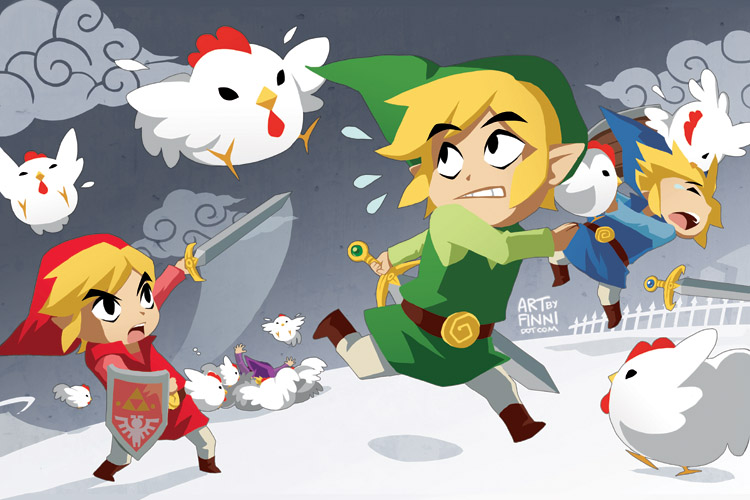
\includegraphics[width=0.6\textwidth]{figures/Sample/tumblr_static_eaceks0rfxsss8o4swscw40wo.jpg}
    \caption[Single Figure Environment Listed Title]{This is a single figure 
    environment}
    \label{fig_singleenv}
\end{figure}

This is a multi-image figure with a top (Figure~\ref{fig_multienv_1}) and bottom (Figure~\ref{fig_multienv_2}) aligned subfigures:

\begin{figure}[ht]
	\centering
	\begin{subfigure}[t]{\textwidth}
		\centering
		
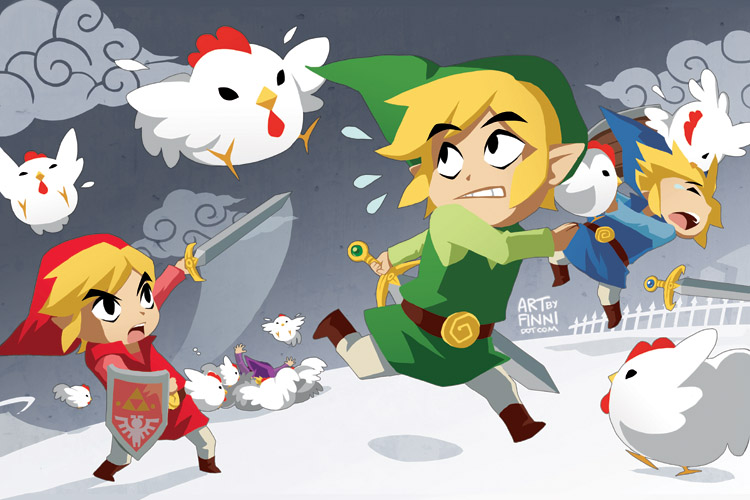
\includegraphics[width=0.7\textwidth]{figures/Sample/tumblr_static_eaceks0rfxsss8o4swscw40wo.jpg}
		\caption{Figure 1}
		\label{fig_multienv_1}
	\end{subfigure}
	~
	\begin{subfigure}[t]{\textwidth}
		\centering
		
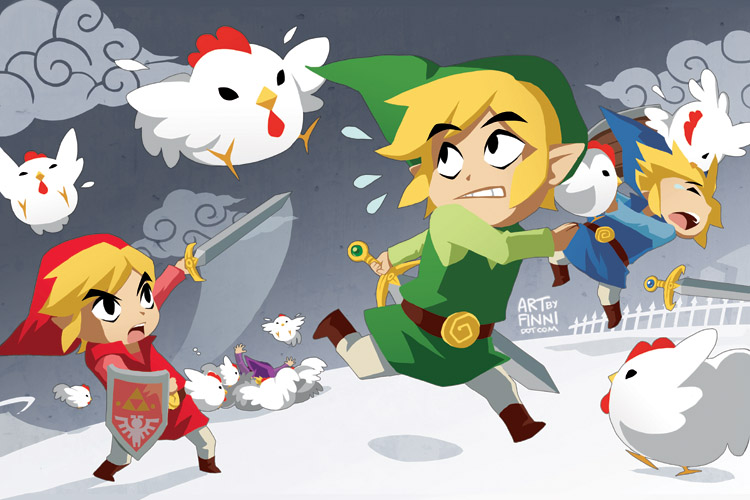
\includegraphics[width=0.7\textwidth]{figures/Sample/tumblr_static_eaceks0rfxsss8o4swscw40wo.jpg}
		\caption{Figure 2}
		\label{fig_multienv_2}
	\end{subfigure}
	
	\caption{A Multi-Figure Environment}
	\label{fig_multienv}
\end{figure}

\section{Tables}

Here is a sample table (Table~\ref{tab_sample}):

	\begin{table}[ht]
	\centering
	\begin{tabular}{ m{0.2\textwidth} m {0.1\textwidth} m{0.15\textwidth} }
		\toprule
		A & $\longleftrightarrow$ & B \\
		C & $\longleftrightarrow$ & D \\
		\bottomrule	
	\end{tabular}	
	\caption{A sample table}	
	\label{tab_sample}
\end{table}

\subsection{Long Tables}
A sample long table is shown in Appendix~\ref{appendix_b}.

\section{Equations}

Here is a sample equation (Equation~\ref{eq_lineslope}):

\begin{equation} \label{eq_lineslope}
	y = mx + b
\end{equation}                  
       \setcounter{figure}{0}
       \setcounter{equation}{0}
       \setcounter{table}{0}

  \chapter{Conclusion}
An ODE is a type, and it exists in many forms. Previously to this research, the Drasil Framework had no flexible and reusable structure for capturing ODE information. The Drasil teams have to manually extract useful information from the original ODE to instruct the Drasil Code Generator to generate code. This approach propagates duplicated information and loses traceability. The newly created structure, \verb|DifferentialModel|, stores linear ODE information based on the conventional matrix concept. It provides the flexibility to transform a linear ODE from one form to another mathematically equivalent form. Once we capture the knowledge of ODE in the new structure, we can reuse it for other purposes, such as producing the numerical solution and displaying the ODE.

Along with \verb|DifferentialModel|, four selected external libraries are responsible for producing the numerical solution for a system of first-order ODEs. Drasil users can get a numerical solution by choosing an algorithm. Currently, although the Calculations module outputs a finite stream of real numbers, $\mathbb{R}^m$, there are other design options. The C\# OSLO provides an option to output an infinite stream of real numbers, $\mathbb{R}^{\infty}$. It has richer data than $\mathbb{R}^m$. Also, outputting the ODE as a function that can return the value of the dependent variable for any value of the independent variable could help generate libraries in Drasil. We did not complete implementing the new specifications for this, but the analysis provides a starting point for future research.

\verb|DifferentialModel| provides reusable ODE information, and external libraries provide mathematical knowledge for solving the ODE. Before we bridge the gap between \verb|DifferentialModel| and external libraries, we enable solving any higher-order ODEs with manually written equations via external libraries. The Double Pendulum case study demonstrates the Drasil Framework can generate code that solves a system of higher-order non-linear ODEs. With all implementations, we are ready to bridge the gap by automating the process of extracting useful information from \verb|DifferentialModel| and then forming an \verb|ODEInfo|. While we are solving a single higher-order linear ODE, we generate it instead of manually writing \verb|ODEInfo|. The automation removes the duplicated information and potentially increases traceability.

This research accomplishes three main goals. Firstly, we capture the knowledge of ODE in a flexible and reusable structure. Secondly, we expand the Drasil capability to solve any higher-order ODEs with manually written equations. The last one is removing the duplicated information caused by the implementation of solving ODEs.

        \setcounter{figure}{0}
        \setcounter{equation}{0}
        \setcounter{table}{0}

\begin{appendix}
    \chapter{Your Appendix}
\label{appendix_a}

This appendix provides detailed explanations of various parts of DifferentialModel.

\section{Constructors of DifferentialModel}
\label{const_de}

% \begin{listing}[ht]
\begin{haskell1}
-- $K_d$ is qdDerivGain
-- $y_t$ is opProcessVariable
-- $K_p$ is qdPropGain
-- $r_t$ is qdSetPointTD
imPDRC :: DifferentialModel
imPDRC = makeASingleDE
	time
	opProcessVariable
	lhs
	rhs
	"imPDRC"
	(nounPhraseSP "Computation of the Process Variable as a function of time")
	EmptyS
	where 
	lhs = [exactDbl 1 `addRe` sy qdDerivGain $* (opProcessVariable $^^ 1)]
	$+ (exactDbl 1 $* (opProcessVariable $^^ 2))
	$+ (exactDbl 20 `addRe` sy qdPropGain $* (opProcessVariable $^^ 0))
	rhs = sy qdSetPointTD `mulRe` sy qdPropGain
\end{haskell1}
\captionof{listing}{Using input language for the example~\ref{eq_odeexmaple} in DifferentialModel}
% \label{code_scexinputl}
% \end{listing}

% \begin{listing}[ht]
\begin{haskell1}
imPDRC :: DifferentialModel
imPDRC = makeASystemDE
	time
	opProcessVariable
	coeffs = [[exactDbl 1, exactDbl 1 `addRe` sy qdDerivGain, exactDbl 20 `addRe` sy qdPropGain]]
	unknowns = [2, 1, 0]
	constants = [sy qdSetPointTD `mulRe` sy qdPropGain]
	"imPDRC"
	(nounPhraseSP "Computation of the Process Variable as a function of time")
	EmptyS
\end{haskell1}
\captionof{listing}{Explicitly set values for the example~\ref{eq_odeexmaple} in DifferentialModel}
% \label{code_scexmatrix}
% \end{listing}

\section{Numerical Solution Implementation}
\label{numsol}

% \begin{listing}[ht]
\begin{python1}
def func_y_t(K_d, K_p, r_t, t_sim, t_step):
    def f(t, y_t):
        return [y_t[1], -(1.0 + K_d) * y_t[1] + -(20.0 + K_p) * y_t[0] + r_t * K_p]
    
    r = scipy.integrate.ode(f)
    r.set_integrator("dopri5", atol=Constants.Constants.AbsTol, rtol=Constants.Constants.RelTol)
    r.set_initial_value([0.0, 0.0], 0.0)
    y_t = [[0.0, 0.0][0]]
    while r.successful() and r.t < t_sim:
        r.integrate(r.t + t_step)
        y_t.append(r.y[0])
    
    return y_t
\end{python1}
\captionof{listing}{Source code of solving PDController in Scipy}
% \label{code_pythonscipy}
% \end{listing}

In line 1, \verb|func_y_t| is a function output the numerical solution, and it is a list of numbers. In the line 2, the local function \verb|f| contains ODE. The line 3 shows local function return a list. Since we want to solve a system of ODE, the index one is the first ODE in this system, and the index two is the second ODE this system. By calling \verb|scipy.integrate.ode|, we pack ODE information in the generic interface. The line between 5 and 10, are procedure how to set configuration and collecting results. Theoretically, we can just return the \verb|r| in line 4 to present returning a function of ODE.

% \begin{listing}[ht]
\begin{java1}
public static ArrayList<Double> func_y_t(double K_d, double K_p, double r_t, double t_sim, double t_step) {
	ArrayList<Double> y_t;
	ODEStepHandler stepHandler = new ODEStepHandler();
	ODE ode = new ODE(K_p, K_d, r_t);
	double[] curr_vals = {0.0, 0.0};

	FirstOrderIntegrator it = new DormandPrince54Integrator(t_step, t_step, Constants.AbsTol, Constants.RelTol);
	it.addStepHandler(stepHandler);
	it.integrate(ode, 0.0, curr_vals, t_sim, curr_vals);
	y_t = stepHandler.y_t;

	return y_t;
}
\end{java1}
\captionof{listing}{A linear system of first-order representation in ACM}
% \label{code_javaacm}
% \end{listing}

% \begin{listing}
\begin{cplusplus1}
vector<double> func_y_t(double K_d, double K_p, double r_t, double t_sim, double t_step) {
	vector<double> y_t;
	ODE ode = ODE(K_p, K_d, r_t);
	vector<double> currVals{0.0, 0.0};
	Populate pop = Populate(y_t);
		
	boost::numeric::odeint::runge_kutta_dopri5<vector<double>> rk = boost::numeric::odeint::runge_kutta_dopri5<vector<double>>();
	auto stepper = boost::numeric::odeint::make_controlled(Constants::AbsTol, Constants::RelTol, rk);
	boost::numeric::odeint::integrate_const(stepper, ode, currVals, 0.0, t_sim, t_step, pop);
	
	return y_t;
}	
\end{cplusplus1}
\captionof{listing}{A linear system of first-order representation in ODEINT}
% \label{code_cplusplusodeint}
% \end{listing}

% \begin{listing}[ht]
\begin{csharp1}
public static List<double> func_y_t(double K_d, double K_p, double r_t, double t_sim, double t_step) {
	List<double> y_t;
	Func<double, Vector, Vector> f = (t, y_t_vec) => {
		return new Vector(y_t_vec[1], -(1.0 + K_d) * y_t_vec[1] + -(20.0 + K_p) * y_t_vec[0] + r_t * K_p);
	};
	Options opts = new Options();
	opts.AbsoluteTolerance = Constants.AbsTol;
	opts.RelativeTolerance = Constants.RelTol;
	
	Vector initv = new Vector(new double[] {0.0, 0.0});
	IEnumerable<SolPoint> sol = Ode.RK547M(0.0, initv, f, opts);
	IEnumerable<SolPoint> points = sol.SolveFromToStep(0.0, t_sim, t_step);
	y_t = new List<double> {};
	foreach (SolPoint sp in points) {
		y_t.Add(sp.X[0]);
	}
	
	return y_t;
}
\end{csharp1}
\captionof{listing}{Source code of solving PDController in OSLO}
% \label{code_csharposlo}
% \end{listing}


\section{Algorithm in External Libraries}
\label{alg_externallib}

\begin{table}[ht]
\begin{tabular}{ p{0.2\textwidth} p{0.7\textwidth} }
	\textbf{Name} & \textbf{Description} \\
	\toprule
	\verb|zvode| & Complex-valued Variable-coefficient Ordinary Differential Equation solver, with fixed-leading-coefficient implementation. It provides implicit Adams method (for non-stiff problems) and a method based on backward differentiation formulas (BDF) (for stiff problems).\\ \hline
	\verb|lsoda| & Real-valued Variable-coefficient Ordinary Differential Equation solver, with fixed-leading-coefficient implementation. It provides automatic method switching between implicit Adams method (for non-stiff problems) and a method based on backward differentiation formulas (BDF) (for stiff problems).\\ \hline
	\verb|dopri5| & This is an explicit runge-kutta method of order (4)5 due to Dormand \& Prince (with stepsize control and dense output).\\ \hline
	\verb|dop853| & This is an explicit runge-kutta method of order 8(5,3) due to Dormand \& Prince (with stepsize control and dense output).\\
	\bottomrule	
\end{tabular}	
\caption{Algorithm Options in Scipy~\citep{scipyfun}}	
\label{tab_algscipy}
\end{table}

\begin{table}[ht]
\begin{tabular}{ p{0.27\textwidth} p{0.7\textwidth} }
	\textbf{Name} & \textbf{Description} \\
	\toprule
	\verb|Euler| & This class implements a simple Euler integrator for Ordinary Differential Equations.\\ \hline
	\verb|Midpoint| & This class implements a second order Runge-Kutta integrator for Ordinary Differential Equations.\\ \hline
	\verb|Classical RungeKutta| & This class implements the classical fourth order Runge-Kutta integrator for Ordinary Differential Equations (it is the most often used Runge-Kutta method).\\ \hline
	\verb|Gill| & This class implements the Gill fourth order Runge-Kutta integrator for Ordinary Differential Equations.\\ \hline
	\verb|Luther| & This class implements the Luther sixth order Runge-Kutta integrator for Ordinary Differential Equations.\\ \hline
	\verb|Higham and Hall| & This class implements the 5(4) Higham and Hall integrator for Ordinary Differential Equations.\\ \hline
	\verb|DormandPrince 5(4)| & This class implements the 5(4) Dormand-Prince integrator for Ordinary Differential Equations.\\ \hline
	\verb|DormandPrince 8(5,3)| & This class implements the 8(5,3) Dormand-Prince integrator for Ordinary Differential Equations.\\ \hline
	\verb|Gragg-Bulirsch-Stoer| & This class implements a Gragg-Bulirsch-Stoer integrator for Ordinary Differential Equations.\\ \hline
	\verb|Adams-Bashforth| & This class implements explicit Adams-Bashforth integrators for Ordinary Differential Equations.\\ \hline
	\verb|Adams-Moulton| & This class implements implicit Adams-Moulton integrators for Ordinary Differential Equations.\\
	\bottomrule	
\end{tabular}	
\caption{Algorithm Options in Apache Commons Maths~\citep{apachefun}}	
\label{tab_algacm}
\end{table}

\begin{table}[ht]
\begin{tabular}{ p{0.4\textwidth} p{0.5\textwidth} }
	\textbf{Name} & \textbf{Description} \\
	\toprule
	\verb|euler| & Explicit Euler: Very simple, only for demonstrating purpose\\ \hline
	\verb|runge_kutta4| & Runge-Kutta 4: The classical Runge Kutta scheme, good general scheme without error control.\\ \hline
	\verb|runge_kutta_cash_karp54| & Cash-Karp: Good general scheme with error estimation.\\ \hline
	\verb|runge_kutta_dopri5| & Dormand-Prince 5: Standard method with error control and dense output.\\ \hline
	\verb|runge_kutta_fehlberg78| & Fehlberg 78: Good high order method with error estimation.\\ \hline

	\verb|adams_bashforth_moulton| & Adams-Bashforth-Moulton: Multi-step method with high performance.\\ \hline
	\verb|controlled_runge_kutta| & Controlled Error Stepper: Error control for the Runge-Kutta steppers.\\ \hline
	\verb|dense_output_runge_kutta| & Dense Output Stepper: Dense output for the Runge-Kutta steppers.\\ \hline
	\verb|bulirsch_stoer| & Bulirsch-Stoer: Stepper with step size, order control and dense output. Very good if high precision is required..\\ \hline
	\verb|implicit_euler| & Implicit Euler: Basic implicit routine.\\ \hline
	\verb|rosenbrock4| & Rosenbrock 4: Solver for stiff systems with error control and dense output.\\ \hline
	\verb|symplectic_euler| & Symplectic Euler: Basic symplectic solver for separable Hamiltonian system.\\ \hline
	\verb|symplectic_rkn_sb3a_mclachlan| & Symplectic RKN McLachlan: Symplectic solver for separable Hamiltonian system with order 6.\\
	\bottomrule	
\end{tabular}	
\caption{Algorithm Options in ODEINT~\citep{odeintfun}}	
\label{tab_algodeint}
\end{table}

\begin{table}[ht]
\begin{tabular}{ p{0.2\textwidth} p{0.7\textwidth} }
	\textbf{Name} & \textbf{Description} \\
	\toprule
	\verb|RK547M| & This method is most appropriate for solving non-stiff ODE systems. It is based on classical Runge-Kutta formulae with modifications for automatic error and step size control.\\ \hline
	\verb|GearBDF| & It is an implementation of the Gear back differentiation method, a multi-step implicit method for stiff ODE systems solving.\\
	\bottomrule	
\end{tabular}	
\caption{Algorithm Options in OSLO~\citep{oslofun}}	
\label{tab_algodeint}
\end{table}

        \setcounter{figure}{0}
        \setcounter{equation}{0}
        \setcounter{table}{0}

    \chapter{Long Tables}
\label{appendix_b}

This appendix demonstrates the use of a long table that spans multiple pages.

\begin{center}
\begin{longtable}{P{3cm}P{3cm}P{2.5cm}P{3.5cm}}
\toprule
\hline
\textbf{Col A} & \textbf{Col B} & \textbf{Col C} & \textbf{Col D} \\ \midrule

\endfirsthead
\multicolumn{4}{c}{\textit{Continued from previous page}} \\ \hline
\textbf{Col A} & \textbf{Col B} & \textbf{Col C} & \textbf{Col D} \\ \hline
\endhead
\hline \multicolumn{4}{r}{\textit{Continued on the next page}} \\
\endfoot
\hline
\endlastfoot

A & B & C & D \\ \midrule

A & B & C & D \\ \midrule

A & B & C & D \\ \midrule

A & B & C & D \\ \midrule

A & B & C & D \\ \midrule

A & B & C & D \\ \midrule

A & B & C & D \\ \midrule

A & B & C & D \\ \midrule

A & B & C & D \\ \midrule

A & B & C & D \\ \midrule

A & B & C & D \\ \midrule

A & B & C & D \\ \midrule

A & B & C & D \\ \midrule

A & B & C & D \\ \midrule

A & B & C & D \\ \midrule

A & B & C & D \\ \midrule

A & B & C & D \\ \midrule

A & B & C & D \\ \midrule

A & B & C & D \\ \midrule

A & B & C & D \\ \midrule

\hline
\end{longtable}
\end{center}

        \setcounter{figure}{0}
        \setcounter{equation}{0}
        \setcounter{table}{0}
\end{appendix}

% The bibliography is set up to allow for multiple bib files
\bibliographystyle{ACM-Reference-Format}
\bibliography{references,references_another}

\label{NumDocumentPages}

\end{document}
% ********************************
